\chapter{Benutzerdokumentation}

\section{Installation}

\section{Beispielsitzung}

Nach Start des Programms wird die graphische Benutzeroberfläche angezeigt.
\begin{figure}[H]
\centering
%\hspace{-1.75cm}
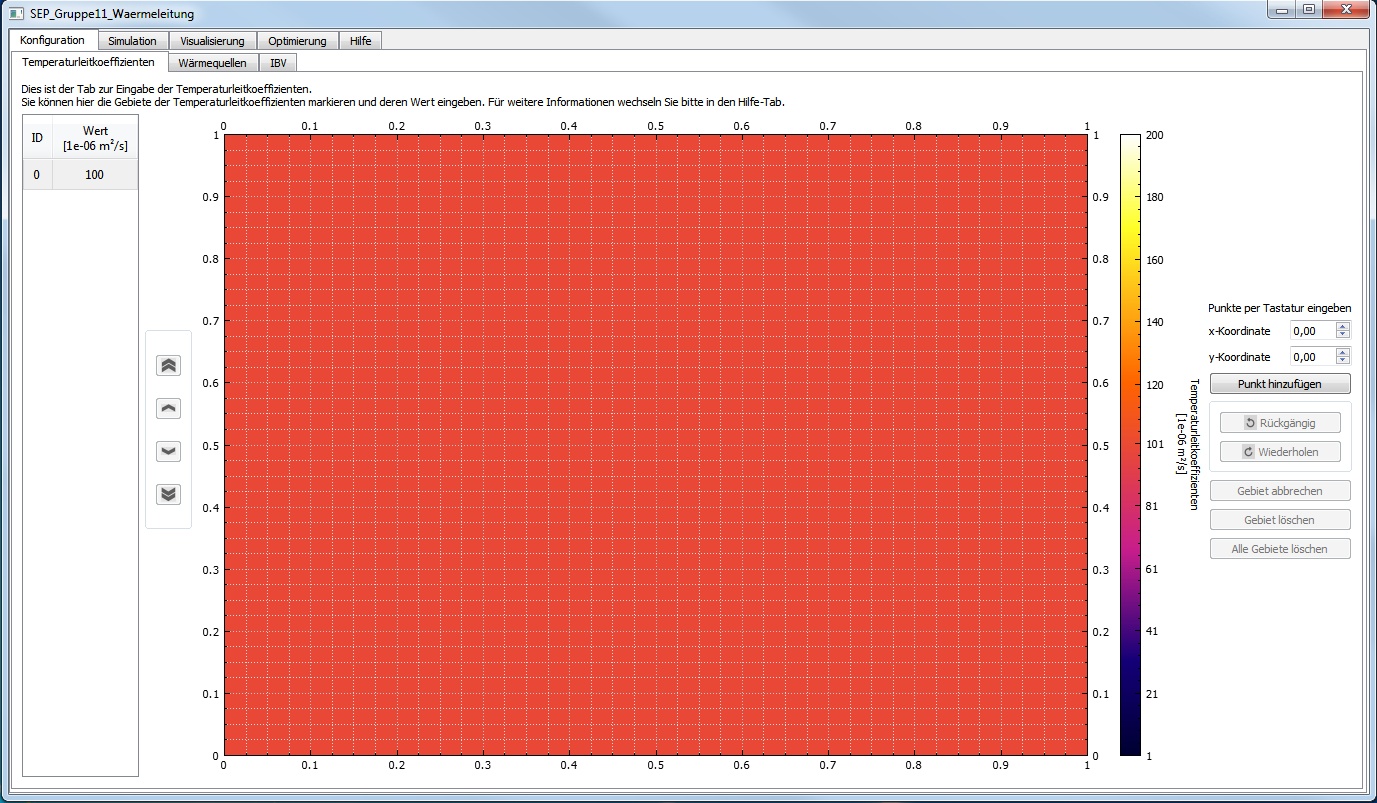
\includegraphics[scale=.5]{Benutzerdokumentation/StartAnzeige.png}\\
\caption{grpaphische Benutzeroberfläche}
\label{grpaphische Benutzeroberfläche}
\end{figure}

\newpage
\noindent
Neues Gebiet hinzufügen:
\begin{figure}[H]
\centering
%\hspace{-1.75cm}
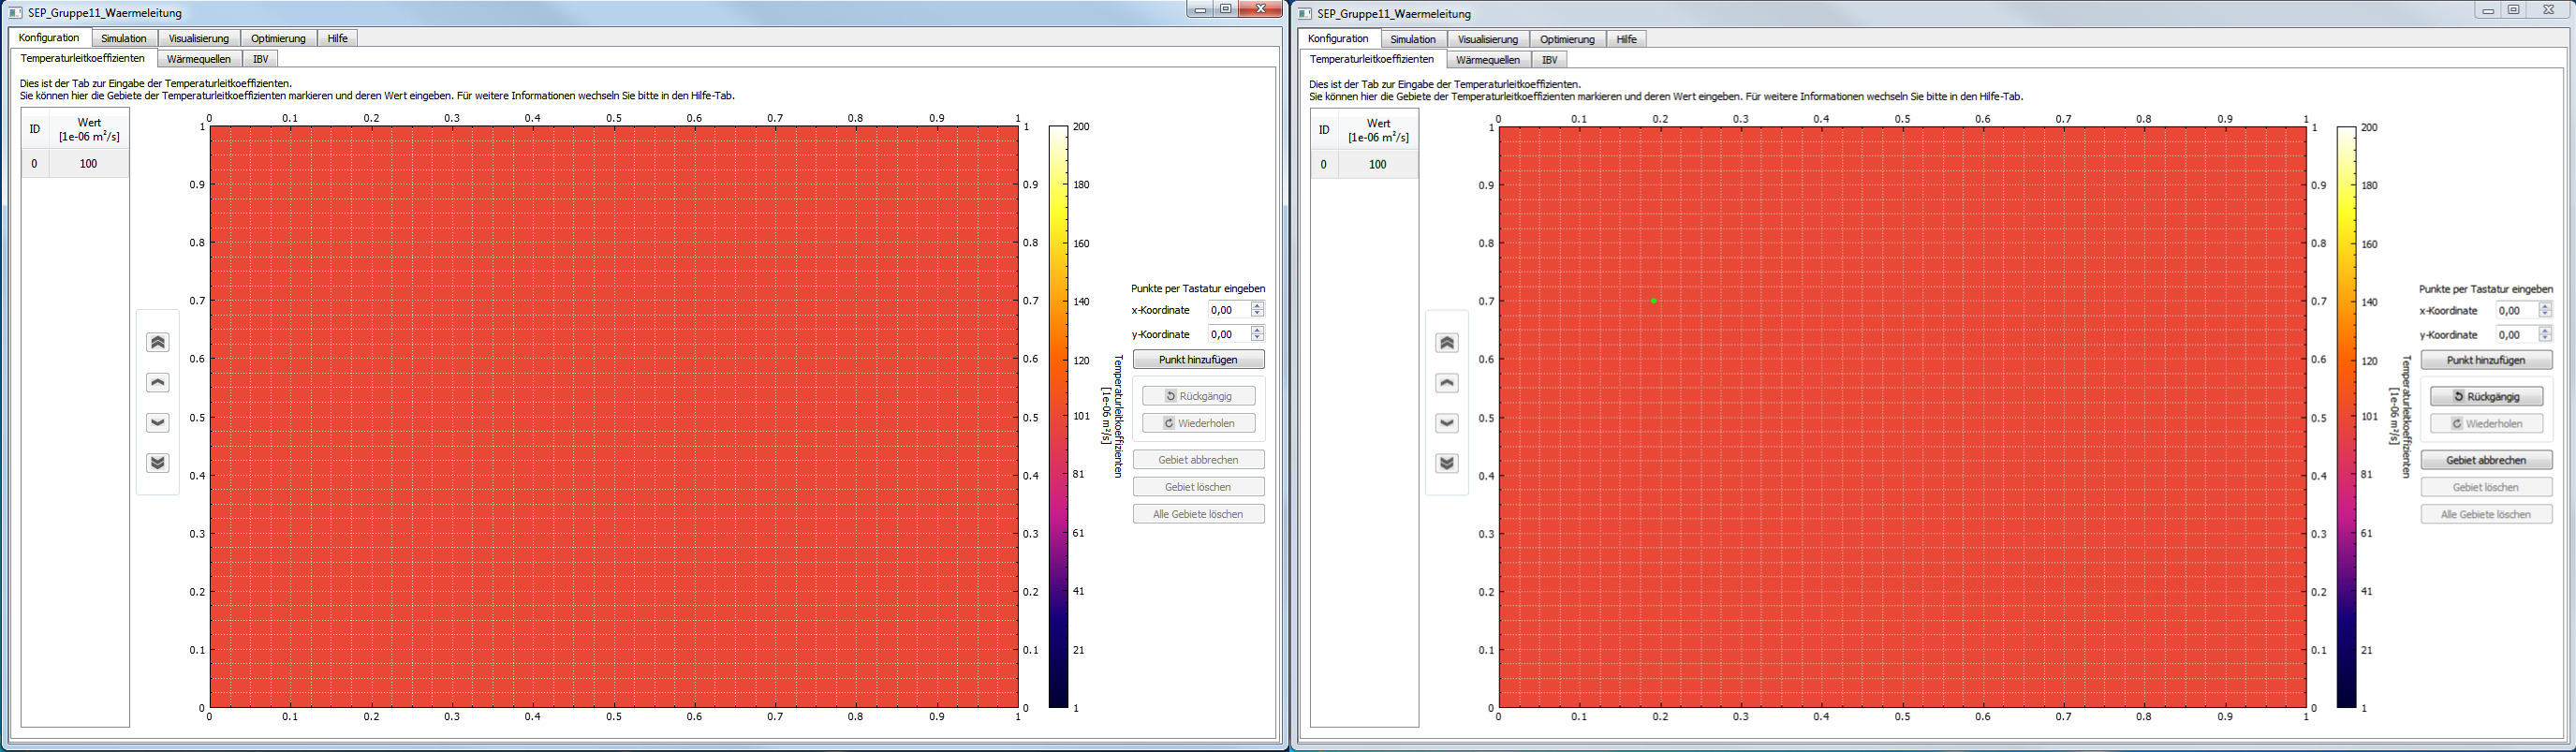
\includegraphics[scale=.25]{Benutzerdokumentation/GebietHinzufuegen1.png}\\
\caption{grpaphische Benutzeroberfläche}
\label{grpaphische Benutzeroberfläche}
\end{figure}

\begin{figure}[H]
\centering
%\hspace{-1.75cm}
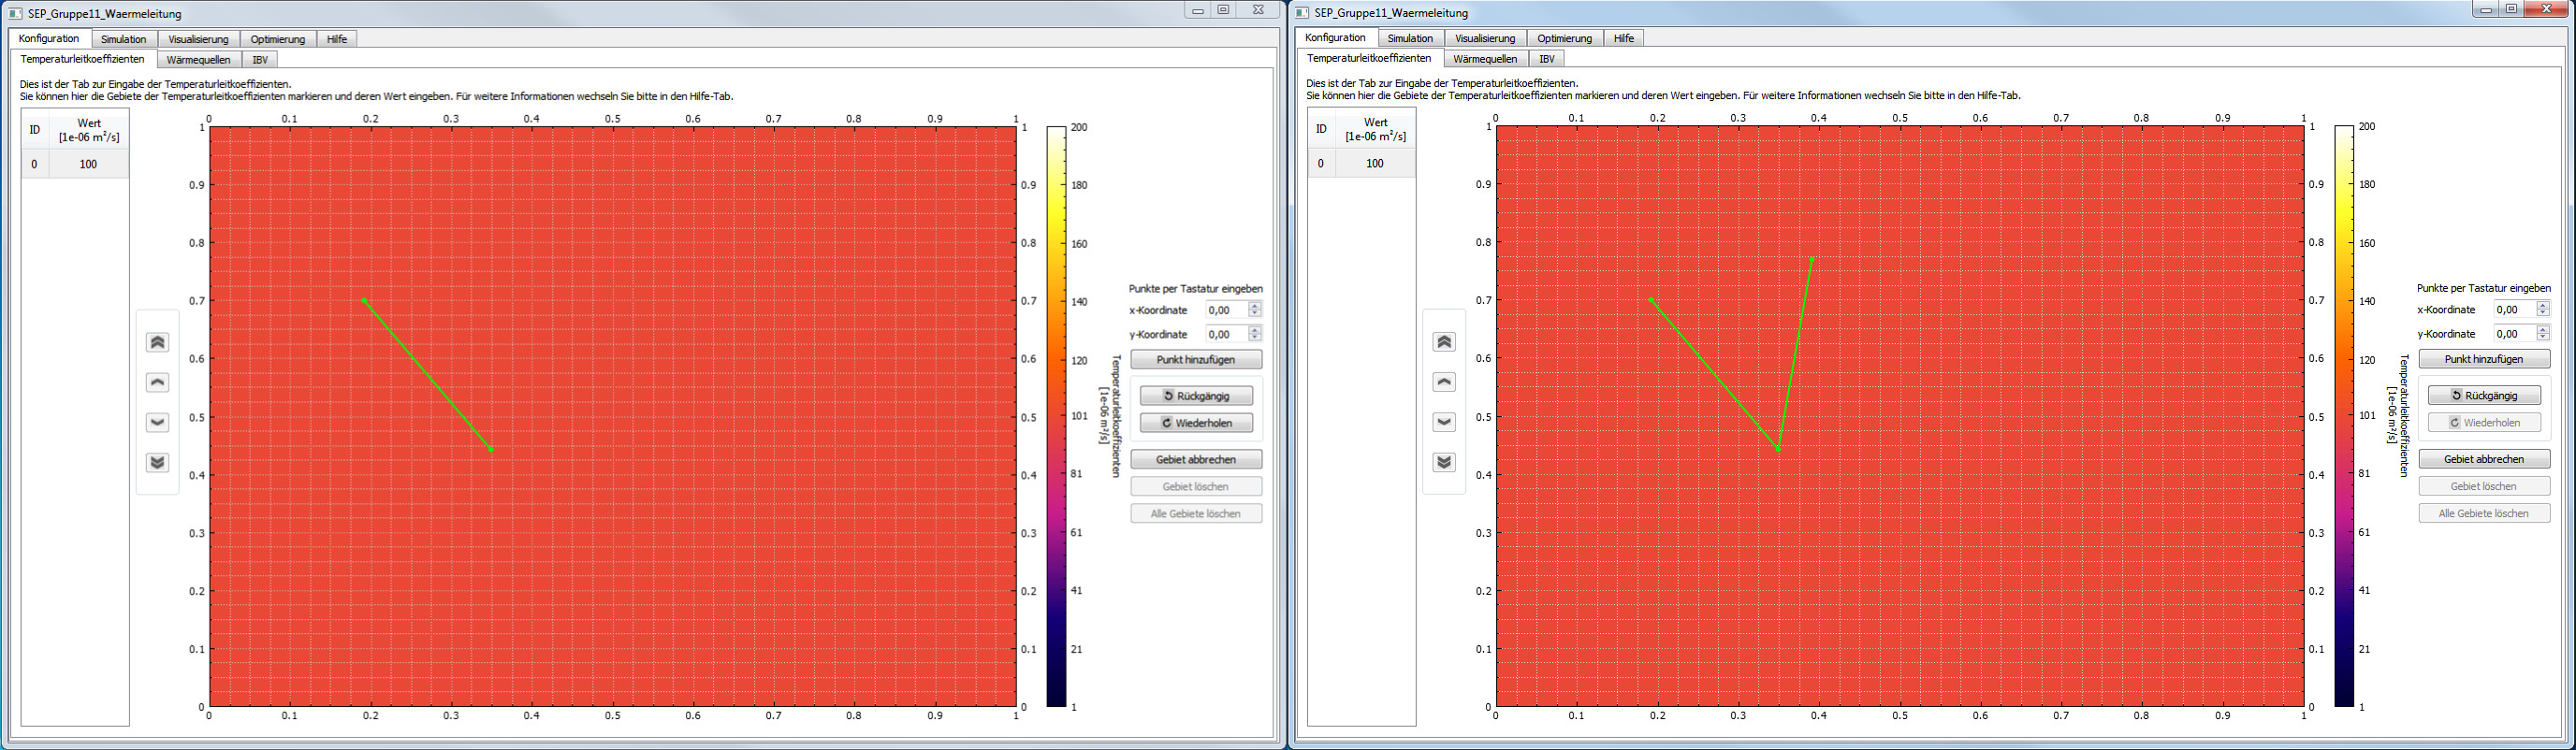
\includegraphics[scale=.25]{Benutzerdokumentation/GebietHinzufuegen2.png}\\
\caption{grpaphische Benutzeroberfläche}
\label{grpaphische Benutzeroberfläche}
\end{figure}

\begin{figure}[H]
\centering
%\hspace{-1.75cm}
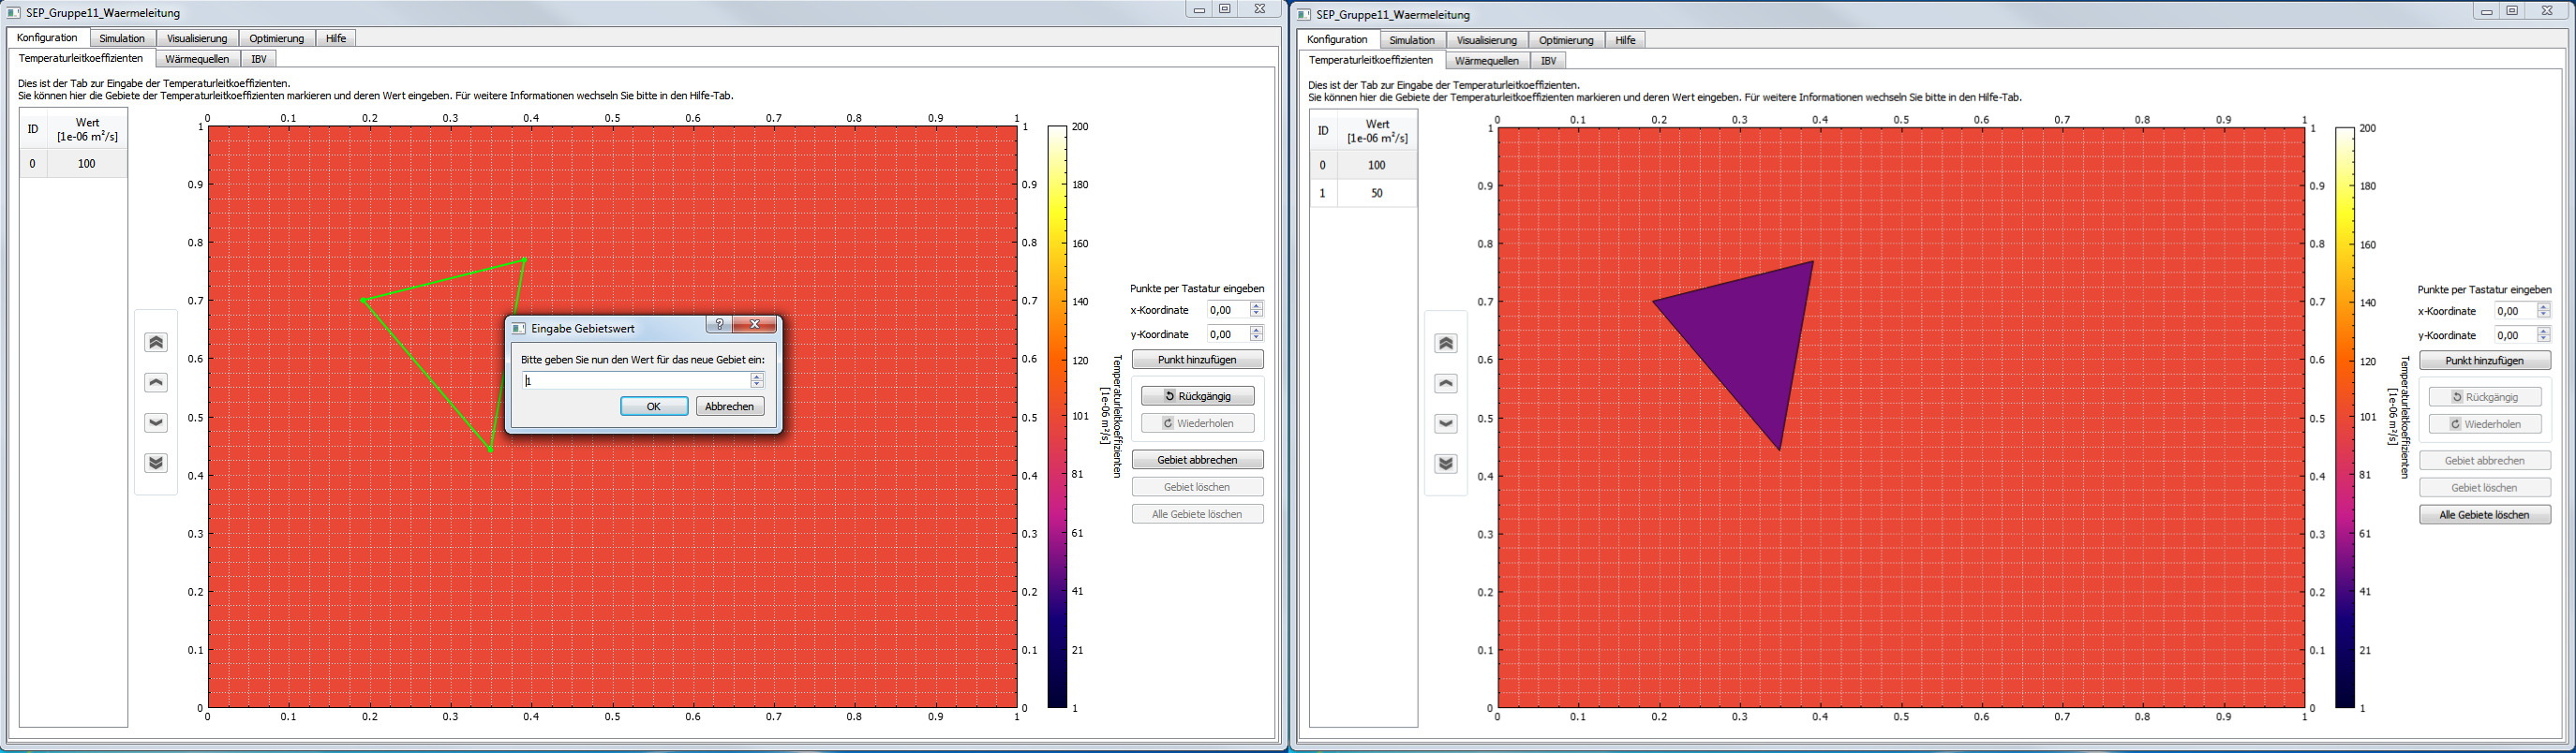
\includegraphics[scale=.25]{Benutzerdokumentation/GebietHinzufuegen3.png}\\
\caption{grpaphische Benutzeroberfläche}
\label{grpaphische Benutzeroberfläche}
\end{figure}